% xelatex

\documentclass[a4paper,10pt]{article}

\usepackage{marvosym}
\usepackage{fontspec} 					%for loading fonts
\usepackage{xunicode,xltxtra,url,parskip} 		%other packages for formatting
\RequirePackage{color,graphicx}
\usepackage[usenames,dvipsnames]{xcolor}
\usepackage{fullpage}                                   % alternative to layaureo
%\usepackage[big]{layaureo} 				%better formatting of the A4 page
%\usepackage{fullpage}					%standard margines
%\usepackage{supertabular} 				%for Grades
\usepackage{titlesec}					%custom \section
\usepackage[none]{hyphenat}				%disable any hyphenation
\usepackage{graphicx}					%photo import
\usepackage{wrapfig}					%image/text wrapping
\usepackage{hyperref}					%setup hyperref package, and colours for links
\usepackage{setspace}					%setup line spacing
\usepackage{array}					%table lines
\usepackage{ulem}					%underlining: for big correct underline distance

\setlength{\parskip}{\baselineskip}

\definecolor{linkcolor}{RGB}{10, 40, 155}
\definecolor{mygray}{gray}{0.25}
\definecolor{linegray}{gray}{0.6}
\definecolor{darkgreen}{RGB}{54, 138, 83}

\def\name{Petar Ivanov}
\def\myline{\color{linegray}\vline}
\def\interestsSpace{\\[1.3mm]}				%wider line spacing

\newcommand{\minorcolor}[1]{\textcolor{mygray}{#1}}
\newcommand{\wide}{\addfontfeature{LetterSpace=3.0}}	%wide letter spacing
\newcommand{\comment}[1]{\small\textcolor{darkgreen}{\,\,//\,#1}}
\newcommand{\mydate}[1]{\minorcolor{\textsc{#1}}}
\newcommand{\bracketcomment}[1]{\small\textit{\minorcolor{(#1)}}}

\hypersetup{
  colorlinks = true,
  urlcolor = linkcolor,
  pdfauthor = {\name},
  pdfkeywords = {Computer Science},
  pdftitle = {\name: Curriculum Vitae},
  pdfsubject = {Curriculum Vitae},
  pdfpagemode = UseNone
}

%FONTS
\defaultfontfeatures{Mapping=tex-text}
\setmainfont[SmallCapsFont = Fontin SmallCaps]{Fontin}

%CV Sections
\titleformat{\section}{\Large\scshape\raggedright}{}{0em}{}[\color{linegray}\titlerule]	% section style
\titlespacing{\section}{0pt}{15pt}{0pt}

% MARGINES
\addtolength{\oddsidemargin}{-3mm}
\addtolength{\evensidemargin}{-3mm}
\addtolength{\textwidth}{8mm}

\addtolength{\topmargin}{5mm}
\addtolength{\textheight}{25mm}

\linespread{1.15}				%line spacing

%--------------------BEGIN DOCUMENT----------------------
\begin{document}
\pagestyle{empty}				% non-numbered pages
\font\fb=''[cmr10]''				%for use with \LaTeX command

% *** Photo ***
\begin{wrapfigure}{r}{4.5cm}
	\setlength\fboxsep{0pt}
	\setlength\fboxrule{0.1pt}
        \vspace{-50pt}\fbox{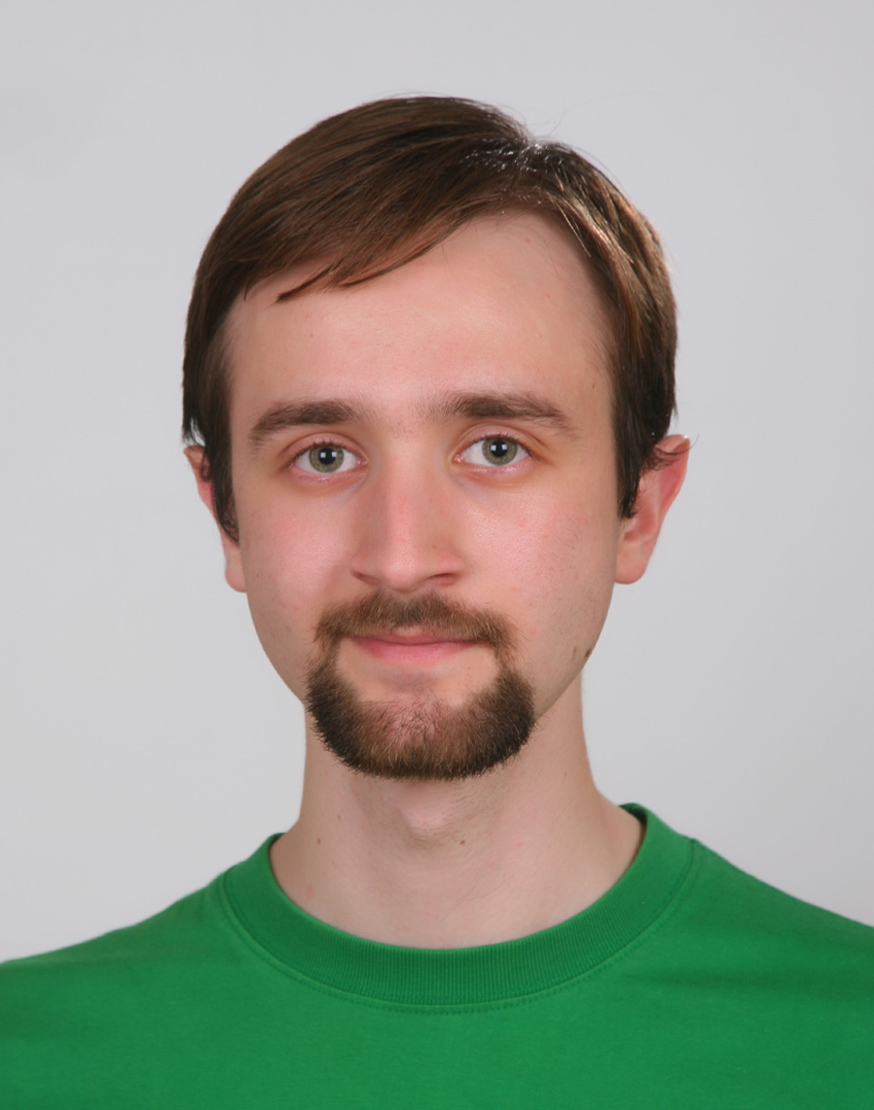
\includegraphics[width=33mm]{PetarIvanov2013.jpg}}
\end{wrapfigure}

% *** Profile ***
\par{\raggedright\Huge\textbf{\vspace{-3mm}\hspace{0mm}\name}}\\		% big name on the top
\vspace{-5mm}{\color{linegray}\rule{10.5cm}{0.1mm}}\\

\hspace{4mm}\begin{tabular}{rl}
        %\minorcolor{Born:} & \textsc{29 May 1989} in Shumen, Bulgaria\\
	%\minorcolor{Address:} & \textsc{14} Georgi Kirkov str., Shumen \textsc{9700}, Bulgaria\\
	\minorcolor{email:} & \href{mailto:peter.ivanov89@gmail.com}{peter.ivanov89@gmail.com}\\
	\minorcolor{site:} & \href{http://pesho.info}{pesho.info}\\
\end{tabular}
\bigskip

%Section: *** Summary ***
\section{Summary}
\begin{center}
  \begin{tabular}{c}
    Informatics competitor, communicator and educator.\\
    Makes the world smarter by pushing algorithms to natural sciencies.
    \end{tabular}
\end{center}


%Section: *** Computer Skills ***
\section{Skills}
\hspace{2.5mm}\begin{tabular}{rp{14cm}}
  Algorithms:     &  Graphs, Combinatorics, Strings, Geometry, Optimization, Dynamic Programming\\
  Languages:      &  \textbf{C\,/\,C++ (STL)}, Python (NumPy, SciPy, MatPlotLib), Ruby, MATLAB, Java\\
        Tools:   &  Unix, Bash, Vim, Git, %HTML\,/\,CSS, 
  {\fb \LaTeX}\\
\end{tabular}
 
%Section: *** Education ***
\section{Education}
\hspace{-2mm}\begin{tabular}{r!{\myline}p{14cm}}
  \mydate{Sep 2013 -- now}     &  Bachelor degree in \textbf{Computer Informatics}\\
\bracketcomment{graduated all semesters}  &  Shumen University, Bulgaria\\
  %\textbf{Faculty of Mathematics and Informatics}

        \multicolumn{2}{c}{}\\
        \mydate{Sep 2011 --- Jun 2013}     &  Master degree \bracketcomment{not accredited} in \textbf{Bioinformatics} \comment{I also taugh algorithms to biologists}\\
	                          &  Yandex School of Data Mining, Moscow, Russia\\
	
        \multicolumn{2}{c}{}\\
        \mydate{Sep 2009 --- Jun 2013}     &  Specialist degree \bracketcomment{equivalent to Master} in \textbf{Applied Mathematics and Informatics}\\
        \bracketcomment{interrupted by visa issues} & Moscow State University, Russia \comment{more calculus}\\
                                  %&  Major in Computer vision at \textsc{Graphics \& Media laboratory}\\
                                  %&  \textbf{Faculty of Computational Mathematics and Cybernetics}\\

	\multicolumn{2}{c}{}\\
        \mydate{Sep 2008 --- Jun 2009}     &  Bachelor degree in \textbf{Computer science} \comment{instructor of advanced algorithmics course}\\
        \bracketcomment{moved in Moscow University} &  %\textbf{Faculty of Mathematics and Informatics},
        Sofia University, Bulgaria \comment{mainly discrete maths}\\
        %{\small\textit{after the first year)}} 
	
	\multicolumn{2}{c}{}\\
        \mydate{Sep 2000 --- Jun 2008}     &  Mathematics and Physics class \comment{award for most scientific achievements of his year}\\
                                  &  Shumen High school of Sciences, Bulgaria\\
%\small\textit{
\end{tabular}
\par\smallskip

%\hspace{7mm}\textit{\minorcolor{\underline{Core courses passed:}}}
%
%\hspace{1.5mm}\begin{tabular}{r!{\myline}p{5cm}r!{\myline}p{6cm}}
%     \minorcolor{Technical}  &  \textsc{Image Processing} & & \\
%       \minorcolor{courses}  &  \textsc{Video Processing} & & \\
%              & \textsc{Computer Vision}\\
%              & \textsc{Combinatorial Optimization}\\
%              & \textsc{Bioinformatics Tools}\\
%              & \textsc{Computational Geometry}\\
%              & \textsc{Computational Linguistics}\\
%\end{tabular}
%
%\hspace{1.5mm}\begin{tabular}{r!{\myline}p{7cm}}
%  \minorcolor{Biological}  &  \textsc{Algorithms in bioinformatics} {\small\textit{(x2)}}\\
%  \minorcolor{courses}  &  \textsc{Molecular Biology} {\small\textit{(x2)}}\\
%                            &  \textsc{Microevolution}\\
%                            &  \textsc{Macroevolution}\\
%                            &  \textsc{Immunology}\\
%                            &  \textsc{Embryology}\\
%\end{tabular}

\hspace{7mm}{\textit{\minorcolor{\underline{Additional:}}}

\hspace{0mm}\begin{tabular}{r!{\myline}p{14cm}}
	\mydate{Jan 2011}       &  \textsc{Vision and Machine-learning Research School}, ENS Lyon, France\\
	\mydate{Jul 2008}       &  \textsc{Russian Summer Informatics Camp}, Sudislavl', Kostroma region, Russia\\
	\mydate{Aug 2007}       &  \textsc{Physics Camp}, Panitsite region, Bulgaria\\
	\mydate{2004 --- 2007}   &  \textsc{Summer Research Informatics Camp}, Varna, Bulgaria\\
	\mydate{2001 --- 2008}   &  \textsc{Mathematics and Informatics Private School ``A\&B''}, Shumen, Bulgaria\\
\end{tabular}

\newpage

%Section: *** Work Experience ***
\section{Work Experience}
\hspace{0mm}\begin{tabular}{r!{\myline}p{14cm}}
        %\multicolumn{2}{c}{}\\
  \mydate{Nov 2013 ---}      &  High-school \textbf{students trainer} for informatics competitions\comment{sketched an algorithmic textbook}\\
  \mydate{now} &  \textit{Mathematics and Informatics Private School ``A\&B''}, Shumen, Bulgaria\\ % (\href{http://ab-bg.com/}{ab-bg.com})\\

        \multicolumn{2}{c}{}\\
        \mydate{Nov 2013 ---}      &  Technical Assistant in online bioinformatics \textbf{\href{https://www.coursera.org/course/bioinformatics}{Coursera}} course \\
        \mydate{Jan 2014} &  \textit{supervised by Dr. Pavel Pevzner}, University of California, San Diego\\

        \multicolumn{2}{c}{}\\
        \mydate{Jul 2013 ---}      &  Summer internship on \href{http://bioinf.spbau.ru/spades}{SPAdes} genome open source assembler \comment{\href{http://pesho.info/wp-content/uploads/chimeras-final.pdf}{presentation}}\\
                 \mydate{Aug 2013} & \comment{proof of concept: used replication bugs to enhence assembly in opensource assembler}\\
                                   &  \textit{supervised by Dr. Pavel Pevzner}, \href{http://bioinf.spbau.ru/}{\textbf{Algorithmic Biology Lab}}, Petersburg Academic University\\

        \multicolumn{2}{c}{}\\
	\mydate{Sep 2012 ---}      &  Microbiological models designer\\
        \mydate{Jun 2013}  &  \textit{supervisor: prof. Konstantin Severinov},  \href{http://www.genebiology.ru/}{Institute of Gene biology}, Russian Academy of Sciences\\
	
        \multicolumn{2}{c}{}\\
        \mydate{Jul 2012 ---}      &  \textbf{Researcher internship} on verification of probabilistic biological models \comment{\href{https://docs.google.com/document/d/1tNkXLaWY3ooA4MEnrbrL2_DOpOaiTlLoFblwzKFZdy0/edit?usp=sharing}{summary}}\\
        \mydate{Aug 2012} &  supervised by Prof. Martin Vechev, \href{http://www.srl.inf.ethz.ch/}{Software Reliability Lab}, ETH Zurich\\
	
        \multicolumn{2}{c}{}\\
        \mydate{Jul 2011 ---}      &  \textbf{\href{http://code.google.com/soc/}{Google Summer of Code}} internship\comment{implemented topological operators on tetrahedral meshes}\\
        \mydate{Aug 2011}         &  Computational Geometry Algorithms Library (\href{http://www.cgal.org/}{CGAL})\\
	
        \multicolumn{2}{c}{}\\
	\mydate{Aug 2010}         &  \textit{Lecturer at school students informatics camp}\\
	                          &  \textbf{\href{http://lksh.ru/}{Russian Summer Informatics Camp}}, Saratov\vspace{-5mm}\\
	
	\multicolumn{2}{c}{}\\
	\mydate{Mar 2008 ---}      &  \textit{Assistant in \textsc{``Design and Analysis of Algorithms''} course}\\
	\mydate{Jun 2009}        &  \textbf{Faculty of mathematics and informatics, Sofia University}, Bulgaria\\

	\multicolumn{2}{c}{}\\
	\mydate{Sep 2008 ---}     &  \textit{Jury, organizer, tester and \textit{author} of the problems in}\\
        \mydate{Jun 2009}        &  \textbf{\href{http://konkurs.musala.com/}{Online programming tournament}}, \textbf{Musala Soft}, Bulgaria\\

	\multicolumn{2}{c}{}\\
	\mydate{Sep 2008 ---}     &  \textit{Author of problems in all} \textsc{Bulgarian Tournaments in Informatics}\\
	\mydate{Jun 2009}        &  \textit{Lecturer in the} \textsc{National Informatics Camps}\\
                                  &  \textbf{National Committee in Informatics}, \textbf{Bulgarian Ministry of Education}\\

	\multicolumn{2}{c}{}\\
	\mydate{Jul 2007 ---}     &  \textit{Developer of a bin-packing genetic algorithm for glass cutting optimization}\\
        \mydate{Sep 2007}        &  \textbf{\href{http://telepol.net/telepol.net/}{Telepol Net}}, Bulgaria \comment{my first algorithm in production}\\
	
\end{tabular}
%\vspace{0mm}
%Section: *** References ***
%\section{References}
%\vspace{-6mm}\hspace{11cm}{\minorcolor{\textit{university teachers of mine}}}\\

%\vspace{-3mm}\hspace{-1mm}\begin{tabular}{llp{4.5cm}}
%	{\textbf {Prof. {\large Krassimir Manev}, PhD}} & {\textbf {PhD {\large Dmitriy Vatolin}}} & {\textbf{PhD {\large Anton Konushin}}}\\
%	\textsc{Discrete Mathematics}& \textsc{Video processing and {\addfontfeature{LetterSpace=-14.0}Compression}} & \textsc{Computer Vision}\\
%	\vspace{2mm}
%	\textit{International Committee of IOI} & \textit{Head of MSU Video group} & \textit{Head of MSU Vision group}\\
%	\textbf{Sof{}ia University} & \textbf{Moscow State University} & \textbf{Moscow State University}\\
%	\href{mailto:manev@fmi.uni-sofia.bg}{manev@fmi.uni-sofia.bg} & \href{mailto:dmitriy@graphics.cs.msu.ru}{dmitriy@graphics.cs.msu.ru} & \href{mailto:ktosh@graphics.cs.msu.ru}{ktosh@graphics.cs.msu.ru}\\
%	\textsc{+359 (887) 25-32-11} & \textsc{+7 (903) 762-82-87} & \textsc{+7 (916) 620-31-85}\\
%\end{tabular}

%\smallskip
%\quad \minorcolor{\textit{* \small the references are university teachers of mine}}

\newpage

%Section: *** Awards ***
\section{Awards}
\par{\vspace{-9mm}\hspace{7cm}{\minorcolor{\textit{the competitions are National Bulgarian if nothing else stated}}}}\\

\vspace{-3mm}\hspace{3.5mm}\begin{tabular}{r!{\myline}p{14cm}}
        \textbf{1}\textsuperscript{st} place    &  \textsc{``Minko Balkanski''} \textsc{Competition in Informatics} \textsc{'08}\\
        \textbf{11}\textsuperscript{th} place   &  \textsc{TopCoder High School Finals}, West Lafayette, USA \textsc{'08}\\
  \textbf{1}\textsuperscript{st} place    &  \textsc{Autumn Tournament in Informatics} \textsc{'07}\\
  \textbf{1}\textsuperscript{st} place    &  Student Competition for the \textsc{Dean's cup of Sofia University} \textsc{'07}\\
  \textbf{2}\textsuperscript{nd} place   &  \textsc{International Young Physicists Tournament} \bracketcomment{regional, in team} \textsc{'06}\\
  \textbf{1}\textsuperscript{st} place    &  \textsc{``Rumen Grozdanov''} \textsc{Informatics and Mathematics Tournament} \textsc{'06}\\
  \textbf{1}\textsuperscript{st} place    &  \textsc{Winter Tournament in Informatics} \textsc{'06}\\
\end{tabular}
\medskip

\hspace{3mm}\begin{tabular}{@{•\enskip}p{14.5cm}}
%\setlength{\parindent}{1cm}
	Awarded as a \textbf{National Laureate in Informatics}, Bulgaria \textsc{'08}\\
        Scholarship for \textbf{science achievements} of \href{http://www.afbulgaria.org/}{\textsc{American Foundation for Bulgaria}} \textsc{'07}---\textsc{'08}\\
	Participated in the \textbf{final rounds} of the \textsc{Bulgarian Olympiad in Informatics} \textsc{'05}---\textsc{'08}\\
        Participated in the \textbf{final rounds} of the \href{http://community.topcoder.com/tc?module=Static&d1=tournaments&d2=home}{\textsc{TopCoder High School}}, West Lafayette, USA \textsc{'07}---\textsc{'08}\\
        Participated in the \textbf{final rounds} of ``\href{http://konkurs.musala.com/}{\textsc{Musala Soft and PC Magazine}}'' competition \textsc{'07}---\textsc{'08}\\
%	Participated in the tournament \textsc{Australian Mathematics Trust}, \textsc{'05}---\textsc{'07}\\
%	Scholarship for \textit{excellent grades}, \textsc{'06}, \textsc{'07} and \textsc{'08}\\
\end{tabular}

%\medskip
%\hspace{3mm}\begin{tabular}{@{--- }p{14.5cm}}
%	Scholarship for \textit{science achievements} of \textsc{American Foundation for Bulgaria} in \textsc{'07} and \textsc{'08}\\
%	Scholarship for \textit{excellent grades} in \textsc{'06}, \textsc{'07} and \textsc{'08}\\
%\end{tabular}

%Section: *** Languages ***
%\section{Spoken languages}
%\hspace{1mm}\begin{tabular}{rp{14cm}}
%	\textsc{English:}     &  Upper-Intermediate\\ % {\small\textit{(certified)}}\\
%	\textsc{Russian:}     &  Fluent\\ % {\small\textit{(certified)}}\\
%	\textsc{Bulgarian:}   &  Native\\
%\end{tabular}

%Section: *** Interests and Activities ***
\section{Activities}
\hspace{2mm}\begin{tabular}{@{•\enskip}p{14.5cm}}
%	\setlength{\parindent}{1cm}
%	Scientifically interested in \textsc{Computer Vision, Computational Geometry, Bioinformatics, Machine Learning, Genetic Algorithms}\interestsSpace	
        %Being impressed by Bioinformatics, Synthetic biology, Combinatorial Optimization, Computer Vision, Computational Geometry, Genetics, Machine Learning, Robotics\interestsSpace
        Solve algorithmic problems \comment{\href{http://www.topcoder.com/tc?module=MemberProfile&cr=10205233}{\textsc{TopCoder}}, \href{http://acm.timus.ru/author.aspx?id=30642}{\textsc{Timus}}, \href{http://rosalind.info/users/cheater_no1/}{\textsc{Rosalind}} }\interestsSpace
        Open the mind and the source \comment{\href{https://github.com/petar-ivanov/}{GitHub profile} }\interestsSpace
        Speak English, Russian and Bulgarian\interestsSpace
        Founded a project for describing educational systems by students \comment{\href{http://students-abroad.info/}{students-abroad.info} }\interestsSpace
        %, \href{https://opensnp.org/users/637}{\textsc{genotype}})\interestsSpace
        % including my own \href{http://pesho.info/category/msu}{\textsc{blog}} about Moscow State University\interestsSpace
       % Practising traditional Bulgarian dances and classical ballroom dances.\interestsSpace
        Love to {\wide dance, hike, bike, orienteer} and {\wide run long}\newline
      $\quad$ \comment{ \textbf{42.195km~in~3:43h} --- \href{http://probeg.org/card.php?id=273}{Zelenograd, Russia, Dec 2011} }\newline
      $\quad$ \comment{ \textbf{100km~in~13:19h} --- \href{http://www.vitosha100km.bg/2011/}{Vitosha mountain, Bulgaria, Jul 2012} } \interestsSpace
\end{tabular}

\end{document}
